\section{Thermally-driven cavity flow}
\label{sec_thermally}  

This case was chosen to demonstrate the coupling of enthalpy and momentum equations.
The problem is illustrated in~Fig.~\ref{fig_thermally}. It is a cavity with a
square-shaped cross-section, with differentially heated side walls. Top and
bottom walls are insulated. Buoyancy forces give rise to circular motion of
the fluid inside the cavity. 

%---------------------------%
%                           %
%  Thermally-driven cavity  %
%                           %
%---------------------------%
\begin{figure}[ht]
  \centering
  \setlength{\unitlength}{1mm}
  \begin{picture}( 55, 53)(0,0)
    \thickbox{ 55}{ 53}
    \put(0,0){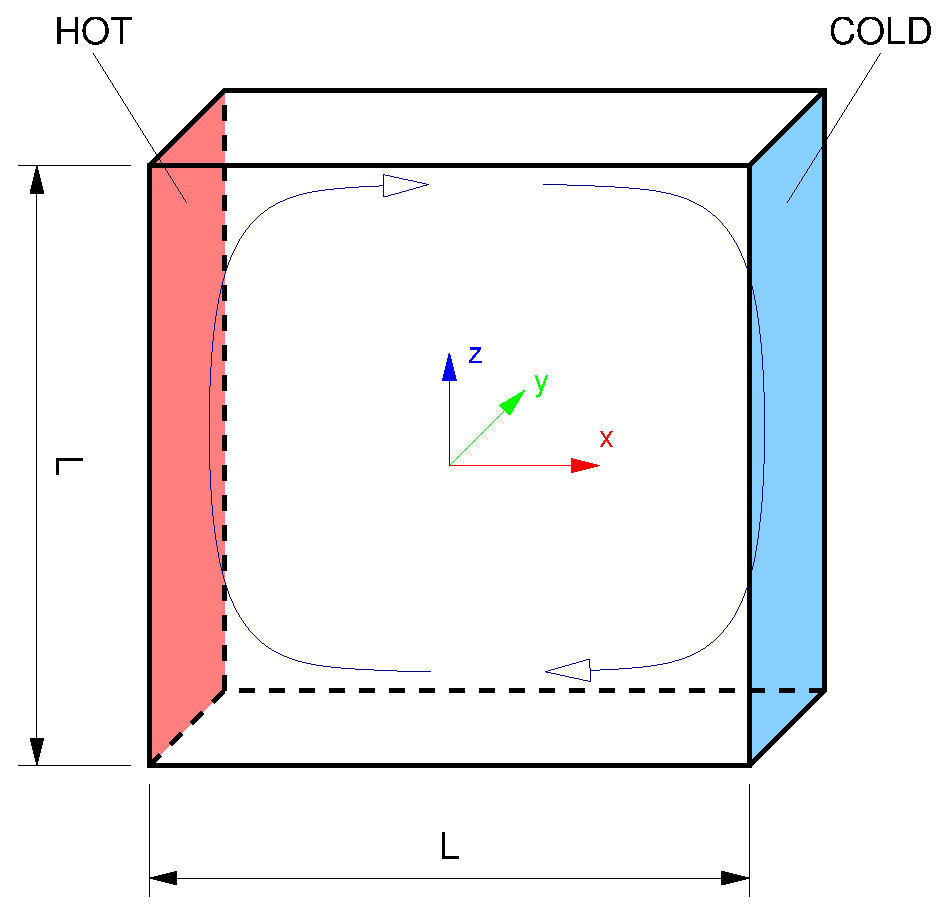
\includegraphics[scale=0.35]{Figures/09-02-thermally.eps}}
  \end{picture}
  \caption{Geometry, boundary conditions and basic topology for the 
           thermally-driven cavity flow.} 
  \label{fig_thermally}
\end{figure}

The program which solves this problem is stored as: {\tt 09-02-main.cpp}.
The features which are new for this problem are described in detail, while the
concepts which have already been explained above (grid generation, boundary
conditions, etc.) are merely mentioned. 

The governing equations in non-dimensional form read:
%
\be
         \int_{V^\s} \frac{\p T^\s}{\p t^\s} dV^\s
       + \int_{S^\s} \uvw^\s T^\s \, d{\bf S}^\s
       = \int_{S^\s} \nabla T^\s \, d{\bf S}^\s
   \label{eq_enthalpy_nd}
\ee
%
\be
         \int_{V^\s} \frac{\p \rho \uvw^\s}{\p t^\s} dV^\s
       + \int_{S^\s} \rho \uvw^\s \uvw^\s \, dS^\s
       = Pr \int_{S^\s} \nabla \uvw \, dS^\s
       - \int_{V^\s} \nabla p^\s \, dV^\s
       + Ra Pr \int_{V^\s} {\bf d} \theta \, dV^\s
   \label{eq_momentum_nd}
\ee
%
if the scales for length, velocity, time and pressure are $L$, ${\alpha}/{L}$
${L^2}/{\alpha}$ and ${\alpha^2 \rho}/{L^2}$ respectively. 
Here~$\alpha = {\lambda}/({\rho C_p)}$ is thermal diffusivity coefficient.
Non-dimensional temperature is defined as 
$T^\s = (T - T_C)/(T_H-T_C)$
%
This problem can be fully characterized with two non-dimensional numbers:
the Rayleigh ($Ra = \rho g \beta \Delta T L^3 / \mu \alpha$) and the 
Prandtl ($Pr = \mu / \alpha \rho$) number. 
These two numbers are defined as a constants at the beginning of the
program:
%
{\small \begin{verbatim}
     10 const real Pr = 0.71;
     11 const real Ra = 1.0e+5;
\end{verbatim}}
%
The problem is two-dimensional, but {\psiboil} can not handle purely two-dimensional
grids. Two-dimensionality can be {\em mimicked} by imposing the periodicity in the
homogeneous direction. This is achieved by the following part of the code:
%
{\small \begin{verbatim}
      4 const real LX =   1.0;
      5 const real LY =   0.125;
      6
      7 const int NX = 64;
      8 const int NY =  4;
     ...
     18   /*----------+
     19   |  grid(s)  |
     20   +----------*/
     21   Grid1D gx( Range<real>( -0.5*LX, 0.5*LX ), NX, Periodic::no());
     22   Grid1D gy( Range<real>( 0, LY ),           NY, Periodic::yes());
     ...
     27   Domain d(gx, gy, gx);
\end{verbatim}}
%
As defined in~Fig.~\ref{fig_thermally}, homogeneous direction is~$y$. The resolution
in $y$ direction is only four cells, a {\em minimum} resolution which can be defined
in {\psiboil}.

For this case, we need variables for temperature, enthalpy source, momentum and its
force, pressure and its source. They are defined with:
%
{\small \begin{verbatim}
     32   Vector uvw(d), xyz(d); // vel
     33   Scalar p  (d), f  (d); // p.
     34   Scalar t  (d), g  (d); // t.
\end{verbatim}}
%
Boundary conditions are defined in lines~39--60, and need no further explanation. 
It is maybe worth reminding that periodic boundary conditions must be set to
variables, notwithstanding they were defined for grids. 

Boundary condition section is followed by the definition of physical properties.
This is a particular case, solved in non-dimensional form 
(Eq.~\ref{eq_enthalpy_nd}~and~\ref{eq_momentum_nd}), so the
only "property" which has to be changed is "dynamic viscosity":
%
{\small \begin{verbatim}
     65   Matter fluid(d);
     66   fluid.mu( Pr );
\end{verbatim}}
%
Setting the number of time steps and selection of Krylov solver are done in 
lines~68 and ~70, and need no further explanation. 
Pressure-Poisson equation, as well as transport equations are defined in lines~75--77:
%
{\small \begin{verbatim}
     75   Pressure pr  ( p,   f,   uvw, time, solver, &fluid);
     76   Momentum ns  ( uvw, xyz,      time, solver, &fluid);
     77   Enthalpy enth( t,   g,   uvw, time, solver, &fluid);
\end{verbatim}}
%
Just before the time loop, multigrid solver is defined in line~79 and
a monitoring location (called {\tt m0}) in line~81:
%
{\small \begin{verbatim}
     79   AC multigrid( &pr );
     80
     81   Location m0("m0", d, NX/2, NY/2, NX/4);
\end{verbatim}}
%

Finally, we reach the time loop, which, in essence, is an {\em evolution} of
the one presented in~Sec.~\ref{sec_cylinder}:
%
{\small \begin{verbatim}
     83   for(time.start(); time.end(); time.increase()) {
     ...
     93     enth.new_time_step();
     94     enth.solve(ResRat(0.001));
     95
     96     ns.cfl_max();
     97     ns.new_time_step();
     98
     99     Comp m = Comp::w();
    100     for_vmijk(xyz,m,i,j,k)
    101       xyz[m][i][j][k] = Pr*Ra * 0.5*(t[i][j][k]+t[i][j][k-1]) * xyz.dV(m,i,j,k);
    102
    103     ns.solve(ResRat(0.001));
    104
    105     multigrid.vcycle(ResRat(0.001));
    106     
    107     ns.project(p);
    108
    109     pr.update_rhs();
    110
    111     m0.print(uvw,Comp::u());
    112   }
\end{verbatim}}
%
Each time step starts with computation of enthalpy. That is possible, because
convective terms are discretized with Adams-Bashforth time stepping scheme, 
meaning that it uses velocity and temperature field in old time step~($n-1$)
and the time step before old~($n-2$). Right-hand side of enthalpy equation
is assembled in line~93, and the linear solver is invoked from line~94.

That is followed by computation of momentum equations. Right hand side terms
depending on old time steps are computed in line~97. For this case, however,
that is not all. Temperature field is coupled with momentum equations
via the Boussinesq approximation defined in lines~99--101. It is worth noting
that macro {\tt for\_vmijk} has been used again, with parameter~{\tt m} specifying
the direction in which the buoyancy acts. It is worth noting
that even for this case, the right hand side is integrated over cell using mid-point
rule, i.e.: multiplying the source with cell volume. Cell volume is stored in
{\tt Vector}'s member function {\tt Vector::dV(m,i,j,k)} which, unlike the {\tt Scalar}'s
variant takes one parameter more, for vector component. The reason for that lies in
the fact that cells of a staggered generally have different volumes than centered cells,
as illustrated in~Fig.~\ref{fig_staggered_cell}.

%------------------%
%                  %
%  Staggered cell  %
%                  %
%------------------%
\begin{figure}[ht]
  \centering
  \setlength{\unitlength}{1mm}
  \begin{picture}( 65, 42)(0,0)
    \thickbox{ 65}{ 42}
    \put(0,0){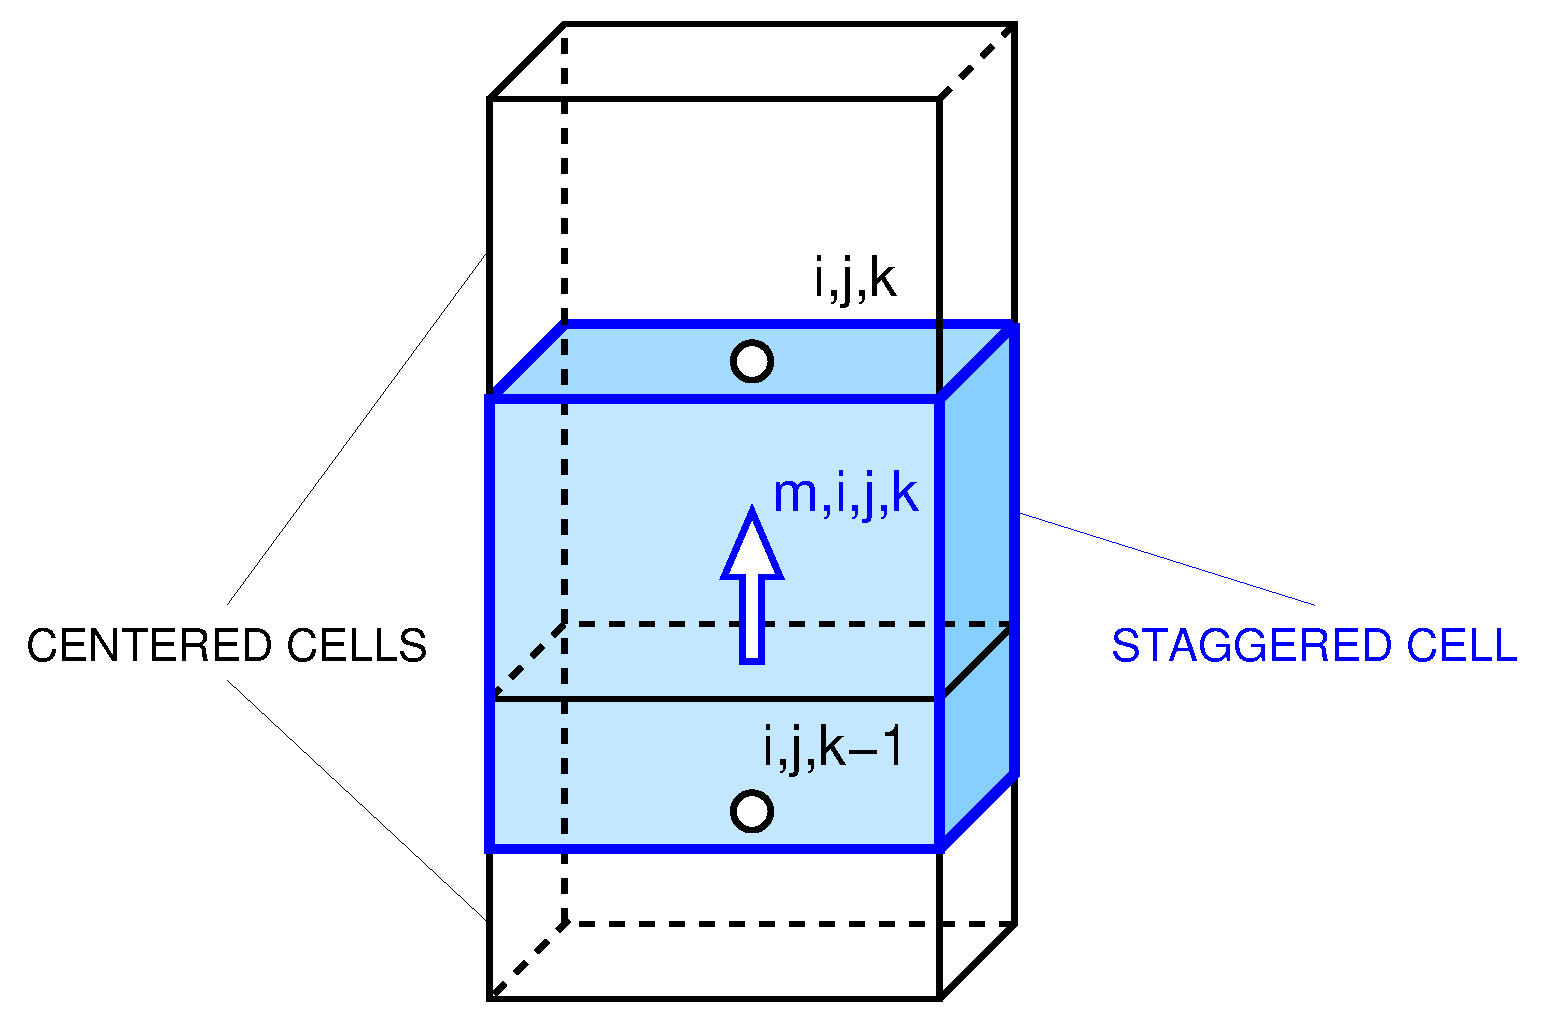
\includegraphics[scale=0.25]{Figures/09-02-staggered-cell.eps}}
  \end{picture}
  \caption{Volume of a staggered ({\tt Vector}'s) cell is different from volume of a 
           centered ({\tt Scalar}'s) cell.
           {\tt Scalar::dV(i,j,k)} $\neq$ {\tt Vector::dV(m,i,j,k)}}
  \label{fig_staggered_cell}
\end{figure}

Figure~\ref{fig_staggered_cell} also makes it clear why temperature for the source
term in program line~101 is taken as an arithmetic average between {\tt t[i][j][k]} 
and {\tt t[i][j][k-1]}.

Lines~103-107 are the same as in~Sec.~\ref{sec_cylinder} and need no explanation. 
A novelty is in line~109, which calls for an explicit update\footnote{It is called 
implicitly from {\tt multigrid.vcycle(ResRat(0.001));}.} of the right-hand side of 
pressure-Poisson equation. It is a trick to  get the mass (im)balance after the
projection of velocities into a divergence-free field. To illustrate it, it is
worth taking a look at the part of the output of this program:
%
{\small \begin{verbatim}
@get_src; err sou = 1.59193 4.2526e-12
Initial  res = 4.68899e-08
Cycle 1; res = 2.01202e-08
Cycle 2; res = 1.61724e-09
Cycle 3; res = 2.19523e-10
Cycle 4; res = 3.98007e-11
Converged after 4 cycles!
@get_src; err sou = 4.37667e-12 6.17362e-14
\end{verbatim}}
%
Compare two lines beginning with {\tt @get\_src}. Te first one is result of implicit
call from line~105, while the last is result of explicit call from line~109. 
Comparing the first number of the two ({\tt 1.59193} and {\tt 4.37667e-12}), 
gives an indication of the success of projection step. In this case, it is
very successful, since projection step reduces mass error by many orders of
magnitude. 

Program line~111 produces time history of $u$ velocity component, plotted 
in~Fig.~\ref{fig_monitor_2}. It is quite convincing that simulation has
reached the steady state. 

%------------------%
%                  %
%  u time history  %
%                  %
%------------------%
\begin{figure}[ht]
  \centering
  \setlength{\unitlength}{1mm}
  \begin{picture}( 75, 52)(0,0)
    \thickbox{ 75}{ 52}
    \put(0,0){\includegraphics[scale=0.3]{Figures/09-02-monitor.eps}}
  \end{picture}
  \caption{Time-history of $u$ velocity component at $x=-0.01$, $y=-0.05$ and $z=-0.26$.}
  \label{fig_monitor_2}
\end{figure}

\subsection{Results and footer output}  

Results, plotted from lines~114--116 (not shown here) are displayed in 
Fig.~\ref{fig_thermally_results}. 

%----------------------------------%
%                                  %
%  Temperature and velocity field  %
%                                  %
%----------------------------------%
\begin{figure}[ht]
  \centering
  \setlength{\unitlength}{1mm}
  \begin{picture}(140, 60)(0,0)
    \thickbox{140}{ 60}
    \put(70, 0){\includegraphics[scale=0.30]{Figures/09-02-velocity.eps}}
    \put( 0, 0){\includegraphics[scale=0.30]{Figures/09-02-temperature.eps}}
  \end{picture}
  \caption{Non-dimensional temperature (left) and velocity field (right) for 
           the thermally driven cavity at $Pr=0.71$ and $Ra=10^5$.}             
  \label{fig_thermally_results}
\end{figure}

Imagine you wanted to extract some profiles from the results, say~$u$~velocity
profile at~$x=0$ and~$w$~velocity profile at~$z=0$. These profiles might be
extracted from Tecplot, which was used to create plots in~Fig.~\ref{fig_thermally_results},
but that will not give the values computed by~{\psiboil}, but rather 
interpolations of these results performed internally by Tecplot. 

{\psiboil} offers a class which can extract profiles from solution, in much the 
same way certain locations in the computational {\tt Domain} are monitored with
the object of type {\tt Location}. The class which extract profiles is called
{\tt Rack}, defined in {\tt Src/Monitor/Rack}, and its usage is demonstrated in lines:
%
{\small \begin{verbatim}
    118   Rack    r0("u-comp", d, NX/2+1, NY/2, Range<int>(1,NX));
    119   Rack    r2("w-comp", d, Range<int>(1,NX), NY/2, NX/2+1);
    120   r0.print(uvw,Comp::u());
    121   r2.print(uvw,Comp::w());
\end{verbatim}}
%
Line~118 creates a measuring {\tt Rack} named {\tt "u-comp"} in {\tt Domain d},
at logical coordinates:~($i$ and~$j$) equal to~{\tt NX/2+1} and~{\tt NY/2} while
ranging in $k$ direction from {\tt 1} to~{\tt NX}. This {\tt Rack} extracts
$u$~velocity component in line~120. 
Line~119 creates a {\tt Rack} oriented in $i$~direction while line~121 extract 
$w$~velocity profile from it. These profiles are printed on 
terminal\footnote{or in a file to which the terminal output was redirected 
with {\tt ./Boil > out \&}} and this printing appears as:
%
{\small \begin{verbatim}
Rack:u-comp
0.0078125 0.046875 -0.492188 -3.7066
0.0078125 0.046875 -0.476562 -10.3498
0.0078125 0.046875 -0.460938 -16.309
0.0078125 0.046875 -0.445312 -21.5107
0.0078125 0.046875 -0.429688 -25.8977
...
\end{verbatim}}
%
which list~$x, y, z$ coordinates, followed by value of $u$~velocity component.
These lists should be extracted from and saved in a separate file. A plot
of these two profiles is shown in~Fig.~\ref{fig_thermally_profiles}.

%-----------------------------%
%                             %
%  u and w velocity profiles  %
%                             %
%-----------------------------%
\begin{figure}[ht]
  \centering
  \setlength{\unitlength}{1mm}
  \begin{picture}(140, 60)(0,0)
    \thickbox{140}{ 60}
    \put( 0, 0){\includegraphics[scale=0.35]{Figures/09-02-u.eps}}
    \put(70, 0){\includegraphics[scale=0.35]{Figures/09-02-w.eps}}
  \end{picture}
  \caption{Non-dimensional $u$~velocity distribution along the line~$x=0$ (left)
           and $w$~velocity distribution along the line~$z=0$.}
  \label{fig_thermally_profiles}
\end{figure}

The profiles in~Fig.~\ref{fig_thermally_profiles} give quantitative data, but
velocity components are not usually reported for this case. It is the Nusselt
number~($Nu = {\p T^\s}/{\p n^\s}$) which is the target 
benchmark datum.
%
As with velocity profiles, it is quite dangerous to extract this value from
post-processing tool, since it is based on internal approximations done in the
tool. The value of $Nu$ which is really computed in {\psiboil} {\em must} be
extracted from the program itself. For this case, it is done with the
following piece of coding:
%
{\small \begin{verbatim}
    123   const int ii = t.si();   /* i inside the domain */
    124   const int iw = ii-1;     /* i in the wall */
    125   const int j  = t.ej()/2; /* j in the middle */
    126   boil::oout << " Nusselt number " << boil::endl;
    127   for_vk(t,k) {
    128     real nu = (t[iw][j][k] - t[ii][j][k]) / t.dxw(ii);
    129     boil::oout << t.zc(k) << " " << nu << boil::endl;
    130   }
\end{verbatim}}
%
%------------------%
%                  %
%  Staggered cell  %
%                  %
%------------------%
\begin{figure}[hb!]
  \centering
  \setlength{\unitlength}{1mm}
  \begin{picture}( 65, 52)(0,0)
    \thickbox{ 65}{ 52}
    \put(0,0){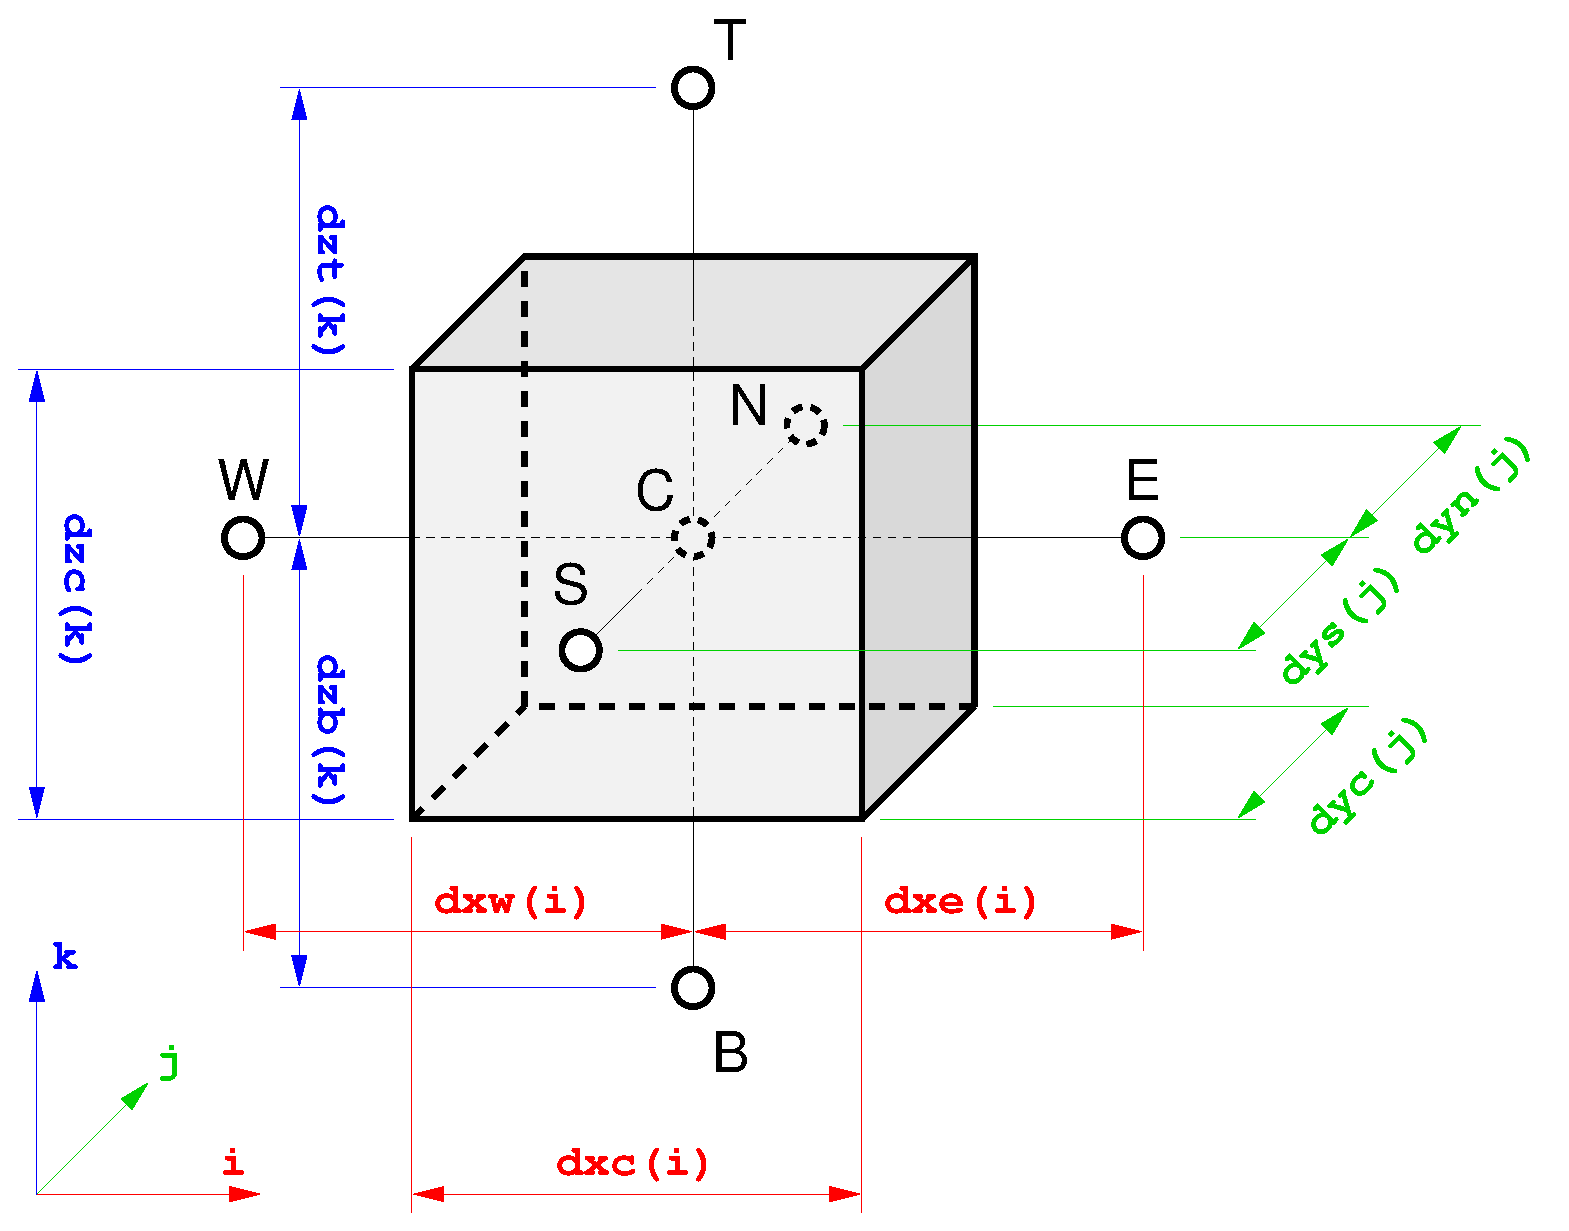
\includegraphics[scale=0.25]{Figures/09-02-cell-dimensions.eps}}
  \end{picture}
  \caption{Cell dimensions.}
  \label{fig_cell_dimensions}
\end{figure}

Lines~123--125 define constants to avoid {\em ghost numbers}. Line~126
just sends a message to the terminal. Loop spanning from line~127 
to~129 computes the $Nu$ and prints it to the terminal, together 
with $z$~coordinate. Here {\tt t[iw][j][k]}  is temperature at the
wall, {\tt t[ii][j][k]} is the temperature in the first computational
cell inside the domain, and {\tt t.dxw(ii)} is the distance between
the cell centre at~$i$ to the cell centre at~$i-1$, which is in {em this
case} at the wall. Distance {\tt dxw(i)} as well as other dimensions
for a general cell (not the one at the wall) are illustrated 
in~Fig.~\ref{fig_cell_dimensions}. 
%
Nusselt number for the heated wall ($x=-0.5$) is plotted in~Fig.~\ref{fig_nusselt}

%------------------%
%                  %
%  Nusselt number  %
%                  %
%------------------%
\begin{figure}[h!]
  \centering
  \setlength{\unitlength}{1mm}
  \begin{picture}( 70, 60)(0,0)
    \thickbox{ 70}{ 60}
    \put( 0, 0){\includegraphics[scale=0.35]{Figures/09-02-nusselt.eps}}
  \end{picture}
  \caption{Non-dimensional $u$~velocity distribution along the line~$x=0$ (left)
           and $w$~velocity distribution along the line~$z=0$.}
  \label{fig_nusselt}
\end{figure}

% \vspace{-20mm}
% \clearpage

%---------------------------------------------------------------------nutshell-%
\vspace*{5mm} \fbox{ \begin{minipage}[c] {0.97\textwidth} %-----------nutshell-%
    {\sf Section \ref{sec_thermally} in a nutshell} \\  %-------------nutshell-%
    
      - If solving a two-dimensional problem with {\psiboil} specify one
      coordinate direction as {\em homogeneous} by making it very thin compared
      to the others and by specifying periodic boundary conditions for it. \\
 
      - Minimum resolution in {\psiboil} is four cells. \\
 
      - When specifying forces for {\tt Momentum} equations, integrate
       them over {\em staggered} volumes ({\tt Vector::dV(m,i,j,k)}). \\
 
      - You can use and additional call to {\tt Pressure::update\_rhs}
      after the projection of velocity, to check the mass conservation
      reduction level. \\
 
      - Extracting profiles from post-processing packages is strongly
      discouraged, since they extract {\em interpolated} solutions, not the
      {\em computed} ones. \\

      - Profiles which are really computed in {\psiboil} can be extracted
      with objects of class {\tt Rack}. \\
 
     - Usage of {\tt Rack} is the same as that of {\tt Location}, except that,
     instead of three coordinates, one sends two coordinates and one {\tt Range}
     to it's constructor. \\

      - You can access all relevant cell dimensions using {\tt Scalar}s member
      functions {\tt dxc}, {\tt dyc}, {\tt dzc}, {\tt dxw}, {\tt dxe},
      {\tt dys}, {\tt dyn}, {\tt dzb} and {\tt dzt}.
 
  \end{minipage} } %--------------------------------------------------nutshell-%
%---------------------------------------------------------------------nutshell-%
